\section{Results}
\subsection{Quantitative analysis}
In this section, we present a quantitative analysis of the results from the studies that were included in the review. The objective of this analysis is to provide an overview of the distribution of authors across different countries and continents (Fig. \ref{fig:geo}), the type of research conducted (Fig. \ref{fig:concept}), and the blockchain technologies employed for each study (Fig. \ref{fig:blockchain}).

\begin{figure}
\centering
\begin{subfigure}{.5\textwidth}
    \centering
    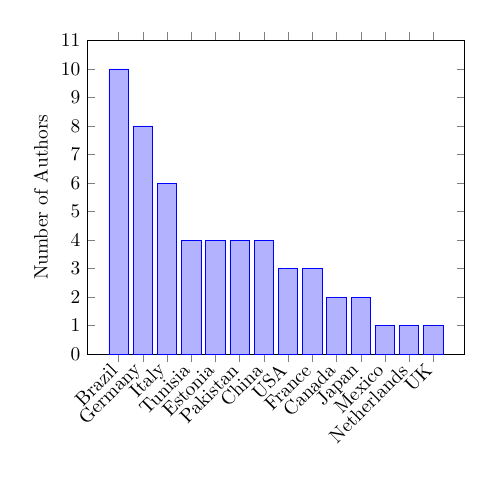
\begin{tikzpicture}[scale=0.7, transform shape]
    \begin{axis}[
        ybar, % create a bar chart
        ylabel={Number of Authors}, % label for the y-axis
        xtick=data, % display tick marks for each data point
        xticklabels={Brazil,Germany,Italy,Tunisia,Estonia,Pakistan,China,USA,France,Canada,Japan,Mexico,Netherlands,UK}, % display the country names for each tick mark
        ymin=0, % set the minimum value for the y-axis to 0
        ymax=11, % set the maximum value for the y-axis to 4
        ytick={0,1,2,3,4,5,6,7,8,9,10,11}, % display tick marks for each integer value on the y-axis
        xticklabel style={rotate=45, anchor=east}, % rotate x-tick labels by 45 degrees and align them to the east
    ]
    \addplot coordinates {(1,10) (2,8) (3,6) (4,4) (5,4) (6,4) (7,4) (8,3) (9,3) (10,2) (11,2) (12,1) (13,1) (14,1)}; % plot the data
    \end{axis}
    \end{tikzpicture}
    \caption{By country}
    \label{fig:geo-country}
\end{subfigure}%
\begin{subfigure}{.5\textwidth}
    \centering
    \begin{tikzpicture}[scale=0.8, transform shape]
    \pie{43.4/Europe,
        18.9/Asia,
        18.9/South America,
        11.3/North America,
        7.5/Africa}
    \end{tikzpicture}
    \caption{By continent}
    \label{fig:geo-continent}
\end{subfigure}%
\caption{Geographic distribution of authors}
\label{fig:geo}
\end{figure}

The intersection between blockchain and BPM has gained interest from multiple nations, with authors based in 14 countries contributing to its research. As can be seen in Fig. \ref{fig:geo-country}, the majority authors were based in the Brazil (10, 18.9\%) followed by the Germany (8, 15.1\%) and Italy (6, 11.3\%), then Tunisia, Estonia, Pakistan, and China (11 each, 7\%). The remaining countries had 3 or less authors who contributed to the selected studies. Brazil in this case is an outlier with 10 authors only working on \citeauthor{alves_exploring_2022} \cite{alves_exploring_2022}. In contrast to the 6 authors from Italy who contributed to both \citeauthor{corradini_engineering_2022} \cite{corradini_engineering_2022} and \citeauthor{corradini_flexible_2022} \cite{corradini_flexible_2022}. The research is mostly concentrated in Europe (43.4\%), Asia and South America (18.9\% each) while North America has 11.3\% as seen in Fig. \ref{fig:geo-continent}. The regions with the least representation are Africa (7.5\%) and Australia with no authors.
\begin{figure}[!h]
    \centering
    \begin{tikzpicture}
    \pie{53.8/Conceptual and empirical,
        46.2/Conceptual,
        0/Empirical}
    \end{tikzpicture}
    \caption{Conceptual vs empirical}
    \label{fig:concept}
\end{figure}

In the context of a SLR, the distinction between conceptual and empirical papers is important because it provides insights into the type of research that has been conducted in the topic of blockchain and BPM. A conceptual paper introduces a new approach or solution that is based on theoretical or conceptual ideas, and normally does not involve any data collection or experimentation \cite{frizzo-barker_blockchain_2020}. An empirical paper, on the other hand, presents research that is based on data collected through observation or experimentation. From our selected studies none of the papers were purely empirical. As can be seen in Fig. \ref{fig:concept}, half of papers were purely conceptual while the other half were both conceptual and empirical at the same time. In the papers featuring both conceptual and empirical elements, first a new solution is introduced. Then, different experiments are run to measure costs (mostly in terms of Ethereum fees \cite{eth}) or performance in comparison to existing solutions.
\begin{figure}
    \centering
    \begin{tikzpicture}
    \pie{61.5/Ethereum,
        38.5/Hyperledger Fabric}
    \end{tikzpicture}
    \caption{Blockchain technology distribution}
    \label{fig:blockchain}
\end{figure}

In our case it is also interesting to see which technologies each study makes use of, which is illustrated on Fig. \ref{fig:blockchain}. As expected Ethereum is the most used platform with 61.5\% of the studies using it. Ethereum is the first and most popular blockchain network that support smart contracts \cite{eth}. The Ethereum network is also permissionless and smart contracts are simple to implement with the Solidity language. In second place comes Hyperledger Fabric \cite{hyperledge}, with 38.5\% of papers developing chaincode solutions. Different from Ethereum, Hyperledger Fabric is a permissioned blockchain platform that is designed for use in enterprise settings \cite{hyperledge}. 
%In contrast to most papers, \citeauthor{ladleif_time_2020} \cite{ladleif_time_2020} was the only study that offered a platform agnostic approach, which they claimed could be applied to Ethereum, Tezos, Hyperledger Fabric and Corda R3.

\subsection{Qualitative analysis and classification results}
In this section, the selected studies are examined in detail and we have grouped them into five different categories, shown in Table \ref{tab:classification}. The categories are based on capabilities that blockchain technologies enables for BPM and challenges faced when implementing such solution. Although the papers are only assigned to one of the categories there is significant overlap between the capabilities supported by the suggested approaches. Here we will only focus on the main topic for each paper.


\setlength{\tabcolsep}{3em}
\begin{table}
    \centering
    \caption{Classification of the selected papers.}
    \begin{tabular}{l c r}
        \hline
        Category & Papers & Number \\
        \hline\hline
        \hyperref[sssec:trust]{Trust Aware} & \cite{alves_exploring_2022, corradini_engineering_2022, fang_workflow_2020, nagano_blockchain_2020, akhtar_blockchain_2020} & 5 (38.4\%)\\
        \hyperref[sssec:flex]{Flexibility} & \cite{corradini_flexible_2022, lopez-pintado_controlled_2022, klinger-upgrade, loukil_decentralized_2021} & 4 (30.8\%)\\
        \hyperref[sssec:temp]{Temporal Constraints} & \cite{abid_modelling_2020, tonga_naha_pupa_2022} & 2 (15.4\%)\\
        \hyperref[sssec:design]{Process Design} & \cite{milani_business_2020, schinle_integration_2020} & 2 (15.4\%)\\
        \hline
    \end{tabular}
    \label{tab:classification}
\end{table}

\subsubsection{Trust Aware}\label{sssec:trust}
Most applications of BC in BPM are introduced into a collaborative setting with multiple parties. Therefore, in these situations the business processes need to be trust aware, meaning to take into account the level of trust between the participants \cite{rosemann2019trust}. \citeauthor{fang_workflow_2020} \cite{fang_workflow_2020} present the Workflow Enactment Service (WES) which allows multiple BPs to interoperate with each other through smart contracts. This eliminates the need for a trusted centralized party. The solution also provides an immutable audit trail for the interoperation of WESs. \citeauthor{alves_exploring_2022} \cite{alves_exploring_2022} suggest a design that combines a Business Process Management System (BPMS) with a blockchain platform into a distributed BPMS to ensure transparent and tamper-proof information sharing among participants. But this solution is later criticized by \citeauthor{nagano_blockchain_2020} \cite{nagano_blockchain_2020} for introducing a Single Point of Trust (SPoT) which a malicious user can attack to falsify related data. They then reveal a system architecture of cross organizational workflow management which eliminates SPoT throughout the workflow lifecycle including defining, executing, and auditing process. \citeauthor{corradini_engineering_2022} \cite{corradini_engineering_2022} intend to target the issue of trust by proposing a novel model-driven methodology for choreography based systems. Their solution, CorChain, relies on a BC infrastructure to enable the trustable execution of a choreography by producing immutable and auditable artefacts. Different from the previous papers, \citeauthor{akhtar_blockchain_2020} \cite{akhtar_blockchain_2020} deals with trust issues stemming from the resources subject to access control policies of multiple organizations. Their approach generates an optimal composite access control policy which enforces all access control policies and minimized policy evaluation cost.

\subsubsection{Flexibility}\label{sssec:flex}
Flexibility refers to the ability of a business to adapt and make changes to its processes quickly and effectively in response to changing requirements \cite{cognini2018business}. Without some degree of flexibility business would not be able to respond to new challenges and opportunities in an ever-changing business environment. Balancing characteristics of blockchain technologies such as immutability with the need for process flexibility has proven to be difficult. \citeauthor{lopez-pintado_controlled_2022} \cite{lopez-pintado_controlled_2022} presents an approach, prototyped in Caterpillar, for dynamic binding of actors to roles in collaborative processes and it also allows actors to control and model subprocesses during runtime. This is accomplished by an off-chain consensus, where all the participants of the collaboration must take part in. Another approach to increasing flexibility was taken by \citeauthor{corradini_flexible_2022} \cite{corradini_flexible_2022}. They propose decoupling the process state, stored in the blockchain as a smart contract, from its execution logic, an off-chain rule-based program. This allows applying runtime changes to a choreography instance without losing the knowledge of the previously exchanged information. Similarly, \citeauthor{klinger-upgrade} \cite{klinger-upgrade} also allow the logic to be updated by decoupling the logic and the data. But differently from the previous solutions they operate only on-chain and rely BPMN collaboration diagram. \citeauthor{loukil_decentralized_2021} \cite{loukil_decentralized_2021} tackles flexibility by proposing an on-chain BPMN interpreter which instantiates and executes processes. This way, they avoid the need for redeployment of the process instance in case of an update to the process model. 

\subsubsection{Temporal Constraints}\label{sssec:temp}
Temporal constraints are the time-based restrictions or rules that govern the execution of a business process. These constraints define the start and end times of activities, the duration of activities, and the time dependencies between activities. Most blockchain technologies have difficulties in ensuring the accurate application of time-based restrictions across a decentralized system since the they do not allow access to an external or internal clock  \cite{ladleif_time_2020}. \citeauthor{abid_modelling_2020} \cite{abid_modelling_2020} tackle the uncertainty of the time it takes to reach transaction finality, which can vary from minutes to hours. They propose an extension to the Caterpillar tool to enable the transformation of temporal constraints for BPMN to smart contract code. In the same vein, \citeauthor{tonga_naha_pupa_2022} \cite{tonga_naha_pupa_2022} seeks to solve the shortcomings of Caterpillar by introducing an extension called Pupa. Pupa not only translates time events but also inclusive gateways to smart contracts.  


\subsubsection{Process Design}\label{sssec:design}
This category includes papers which concern themselves broadly with the design (and modeling) activity of BPM. Designing and modeling processes for blockchain technologies comes with its own challenges because of the idiosyncrasies of the technology. Although all studies selected touch on this topic, the following two papers provide new perspectives which are worth highlighting. \citeauthor{milani_business_2020} \cite{milani_business_2020} analyze the business process redesign (BPR) principles in light of their applicability to blockchain-based solutions. They adapt the best practices of BPR for BC and also explore their applicability with a case study. On a different direction than most papers, \citeauthor{schinle_integration_2020} \cite{schinle_integration_2020} introduces a reverse translator which takes arbitrary chaincode and translates it to a BPMN 2.0 model. Their aim is to enable monitoring of processes defined within a chaincode while reducing the required knowledge about Hyperledger Fabric.